\documentclass[]{exam}
\usepackage{graphicx}
\usepackage{wrapfig}
\usepackage[utf8]{inputenc}

\title{PSYCH 260H Quiz 1}
\author{}
\date{September 8, 2017}

\pagestyle{headandfoot}
\firstpageheader{PSY 260H}{Section 002}{Quiz 1}
\runningheader{PSY 260H}{Section 002}{Quiz 1}
\firstpagefooter{}{Page \thepage\ of \numpages}{}
\runningfooter{}{Page \thepage\ of \numpages}{}

\begin{document}
\maketitle

\begin{center}
  \fbox{\fbox{\parbox{5.5in}{\centering
        Answer the questions using the Scantron form.}}}
\end{center}
\vspace{0.1in}
\makebox[\textwidth]{Name:\enspace\hrulefill}

\newpage

\section{Main - 10 pts}

\begin{questions}


\begin{figure}[h]
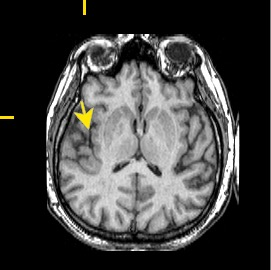
\includegraphics[width=0.4\textwidth]{img/260-2016-09-12-quiz-1-fig-1.jpg}
\centering
\end{figure}

\question The image illustrates what type of slice?
\begin{choices}
\choice Sagittal.
\choice Dorsal.
\choice Coronal.
\correctchoice Axial.
\end{choices}

\question All of the following structures can be seen in the figure EXCEPT
\begin{choices}
\choice Corpus callosum.
\choice Gray matter.
\correctchoice 4th ventricle.
\choice Cerebral cortex.
\end{choices}

\question The figure illustrates the use of \fillin magnetic resonance imaging (MRI), a technique with \fillin spatial resolution.
\begin{choices}
\choice functional; fair ($\sim 3+$ mm).
\correctchoice structural; good ($\sim 1$ mm).
\choice neural; excellent ($\sim 1$ micron).
\choice diffusion tensor; poor ($\sim 1$ cm).
\end{choices}

\question Who believed that the \emph{heart} was the mental organ, and the brain was merely a cooling system for the body?
\begin{choices}
\correctchoice Aristotle.
\choice Galen.
\choice Vesalius.
\choice Descartes.
\end{choices}

\newpage

\question Event-related potentials are detected using \fillin; they measure \fillin.
\begin{choices}
\choice positron emission tomography (PET); local metabolic rates.
\choice magnetic resonance imaging (MRI); the integrity of white matter fiber tracts.
\correctchoice electroencephalography (EEG); the time-locked electrical activity of large numbers of neurons.
\choice magnetoencephalography (MEG); average brain magnetic activity.
\end{choices}

\question The lateral fissure is \fillin to the longitudinal fissure.
\begin{choices}
\choice posterior.
\choice anterior.
\choice rostral.
\correctchoice inferior.
\end{choices}

\question Information about airborne chemicals enters the CNS via the 1st (I) cranial or \fillin nerve and projects to the \fillin.
\begin{choices}
\choice optic; lateral geniculate nucleus.
\correctchoice olfactory; olfactory cortex.
\choice optic; substantia nigra.
\choice oculomotor; superior colliculus.
\end{choices}

% \question All of these structures are components of the forebrain EXCEPT:
% \begin{choices}
% \choice hippocampus.
% \correctchoice tegmentum.
% \choice hypothalamus.
% \choice cerebral cortex.
% \end{choices}

\question All of these structures are components of the midbrain EXCEPT:
\begin{choices}
\choice superior colliculus.
\correctchoice 3rd ventricle.
\choice tegmentum.
\choice inferior colliculus.
\end{choices}

\question Why does fMRI represent an indirect measure of brain activity?
\begin{choices}
\choice It measures brain structure, not function.
\choice It measures electrical activity, but neurons send chemical messages.
\correctchoice It measures changes in blood oxygen and blood flow that follow neural activity.
\choice It has poor spatial resolution.
\end{choices}

% \question Optogenetic neural stimulation techniques are \fillin methods with \fillin spatial and temporal resolution than functional MRI (fMRI).
% \begin{choices}
% \choice structural; higher
% \correctchoice functional; higher
% \choice structural; lower
% \choice functional; lower
% \end{choices}

% \question Which of these landmarks separates the left from the right cerebral hemisphere?
% \begin{choices}
% \choice Lateral fissure
% \correctchoice Longitudinal fissure
% \choice Anterior cingulate gyrus
% \choice Central sulcus
% \end{choices}

% \question Which of these landmarks separates the frontal lobe from the parietal lobe?
% \begin{choices}
% \choice Lateral fissure
% \choice Longitudinal fissure
% \choice Anterior cingulate gyrus
% \correctchoice Central sulcus
% \end{choices}

\question Anterograde and retrograde histochemical tracers help neuroscientists determine \fillin.
\begin{choices}
\choice what stimuli best activate a brain region.
\correctchoice what connects where.
\choice when to stimulate a brain region for maximum effect.
\choice whether a brain area is functioning normally.
\end{choices}

\begin{center}
\bfseries{Turn to the next page to answer the bonus questions.}
\end{center}

\newpage

\section{Bonus}

\question This forebrain structure in the ventral diencephalon controls both the autonomic nervous system and the endocrine system.
\begin{choices}
\choice Hippocampus.
\choice Thalamus.
\choice Medulla.
\correctchoice Hypothalamus.
\end{choices}

\question The arrow in the figure on page 2 shows two parts of the brain that are structurally related and adjacent to one another, the \fillin and the \fillin.
\begin{choices}
\correctchoice lateral fissure; temporal lobes.
\choice spinal cord; lateral ventricles.
\choice amygdala; tectum.
\choice basal ganglia; 4th ventricle.
\end{choices}

\end{questions}

\end{document}
